% Created 2018-06-25 Mo 13:07
% Intended LaTeX compiler: pdflatex
\documentclass[11pt]{scrreprt}
\usepackage[utf8]{inputenc}
\usepackage[T1]{fontenc}
\usepackage{graphicx}
\usepackage{grffile}
\usepackage{longtable}
\usepackage{adjustbox}
\usepackage{wrapfig}
\usepackage{rotating}
\usepackage[normalem]{ulem}
\usepackage{amsmath}
\usepackage{pdfpages}
\usepackage{units}
\usepackage{textcomp}
\usepackage{amssymb}
\usepackage{capt-of}
\usepackage{hyperref}
\usepackage[framemethod=TikZ]{mdframed}
\usepackage[authoryear,round]{natbib}
\title{Response to comments}
\subtitle{Synergistic radar and radiometer retrievals of ice hydrometeors}
\date{}
\hypersetup{
 pdfauthor={Simon Pfreundschuh},
 pdftitle={},
 pdfkeywords={},
 pdfsubject={},
 pdfcreator={Emacs 24.5.1}, 
 pdflang={English}}

\RequirePackage[normalem]{ulem} %DIF PREAMBLE
\RequirePackage{luacolor}\definecolor{RED}{rgb}{1,0,0}\definecolor{BLUE}{rgb}{0,0,1} %DIF PREAMBLE
\providecommand{\DIFadd}[1]{{\protect\textcolor{blue}{\uwave{#1}}}} %DIF PREAMBLE
\providecommand{\DIFdel}[1]{{\protect\textcolor{red}{\sout{#1}}}}                      %DIF PREAMBLE
%DIF SAFE PREAMBLE %DIF PREAMBLE
\providecommand{\DIFaddbegin}{} %DIF PREAMBLE
\providecommand{\DIFaddend}{} %DIF PREAMBLE
\providecommand{\DIFdelbegin}{} %DIF PREAMBLE
\providecommand{\DIFdelend}{} %DIF PREAMBLE
%DIF FLOATSAFE PREAMBLE %DIF PREAMBLE
\providecommand{\DIFaddFL}[1]{\DIFadd{#1}} %DIF PREAMBLE
\providecommand{\DIFdelFL}[1]{\DIFdel{#1}} %DIF PREAMBLE
\providecommand{\DIFaddbeginFL}{} %DIF PREAMBLE
\providecommand{\DIFaddendFL}{} %DIF PREAMBLE
\providecommand{\DIFdelbeginFL}{} %DIF PREAMBLE
\providecommand{\DIFdelendFL}{} %DIF PREAMBLE

\mdfdefinestyle{change}{%
  topline=false,
  leftline=true,
  rightline=false,
  bottomline=false
}

\newenvironment{change}[1][]{%
  \begin{mdframed}[frametitle={Changes starting in line #1:}, style=change]%
}{%
  \end{mdframed}%
}

\begin{document}
\maketitle

\setlength{\parindent}{0cm}

This document contains the responses to the comments of each reviewer followed
by the marked-up differences of the manuscript and the revised version. For each
comment the author's response and, if applicable, the corresponding changes in
the manuscript are listed. Line numbers of changes are given with respect to the
revised manuscript.

In response to the combined comments of the referees, all computations
have been repeated and most of the manuscript has been rewritten. The
following general changes have been implemented:

\begin{itemize}
\item We have switched to an airborne measurement set-up and
   the manuscript has been modified accordingly.
\item The text in the result section has been shortened.
\item Redundant results for scene 2 have been placed in an appendix.
\item The selection of tested retrieval habits has been revised and changed.
\end{itemize}

\chapter{Comments from referee 1}
\section{General comments}

\subsection*{Reviewer comment 1}

The revised manuscript is vastly improved and my concerns have mostly been
satisfied in these revisions. I agree that recasting the measurements as
airborne is an appropriate way to simplify the radiative transfer assumptions
and demonstrate the concept. My second comment, about the inclusion of forward
model error, is not directly addressed though changes in the methods but I do
agree with the author response that such an error would be scene-dependent and
therefore not trivial. However, I think the appropriate caveats have been
mentioned in the interpretation of results so as to not interpret the combined
or radiometer-only methods as being poor compared to the radar due to the higher
chi-squared(y) - in fact, it is noted that the radar is instead overfitting the
measurements.

I only found a few instances of inconsistent nomenclature (e.g., capitalization
of GEM on line 252) that should be corrected prior to publication.

\subsubsection*{Author response}

We would like to thank the auto for pointing out the inconsistencies in nomenclature, which
we will correct in the revised version of the manuscript.


\subsubsection*{Changes in manuscript}

\begin{change}[230]
GEM Graupel, \DIFdelbegin \DIFdel{Gem }\DIFdelend \DIFaddbegin \DIFadd{GEM
}\DIFaddend Hail and GEM Cloud Ice are more efficient.
\end{change}

\chapter{Comments from referee 2}

\section{General comments}

\subsection*{Reviewer comment 1}

L 106: that cloud ice particles are small and abundant while snow particles are
large and much rare is nature not the model. So I would recommend to change the
sentence: " An important characteristic can be identified here.."

\subsubsection{Author response}

The proposed change will be adopted in the revised manuscript.

\subsubsection*{Changes in manuscript}

  \begin{change}[106]
    An important characteristic \DIFdelbegin \DIFdel{of the model }\DIFdelend
    can be identified here, which will help to better understand the retrieval
    results presented later:
  \end{change}

\subsection*{Reviewer comment 2}

 L222-223: The two sentences are a bit contradictiry: Just say M1 results will be shown for certain aspects only

\subsubsection{Author response}

The proposed changes will be adopted in the revised manuscript.

\subsubsection*{Changes in manuscript}

  \begin{change}[220]
 In addition to a two-moment radar-only retrieval, also a one-moment version
 (M1), in which only the $D_m$ parameter is retrieved has been tested.
 \DIFdelbegin \DIFdel{For completeness, retrieval results for IWC will be
   reported also for the M1 version. However, to allow for better comparison
   with the combined and passive-only retrieval , for the remaining results only
   the two-moment version is considered}\DIFdelend \DIFaddbegin \DIFadd{However,
   results of this version will be shown only for the comparison of IWC
   retrieval errors}\DIFaddend .
  \end{change}

\subsection*{Reviewer comment 3}

 L247 WC is used as abbreviation before being defined

\subsubsection{Author response}

We will correct this in the revised manuscript.

\subsubsection*{Changes in manuscript}

  \begin{change}[247]
 Mass backscattering efficiency and attenuation coefficient are defined as the
 ratio of the corresponding cross-section $\sigma$ and the bulk water content
 \DIFaddbegin \DIFadd{(\text{WC})}\DIFaddend :
\begin{align}
  Q &= \frac{\sigma}{\text{WC}}
\end{align}
\end{change}

\subsection*{Reviewer comment 4}

 Figure 5 caption: say that this is an ice cloud

\subsubsection{Author response}

The caption of Fig.~5 will be changed in the revised manuscript as shown below.

\subsubsection*{Changes in manuscript}
 

\begin{change}[284]
Simulated observations of a homogeneous, $5\ \unit{km}$ thick \DIFaddbeginFL \DIFaddFL{ice }\DIFaddendFL cloud
  \DIFdelbeginFL \DIFdelFL{layer }\DIFdelendFL centered at $10\ \unit{km}$ with varying water content $m$ and
  mass-weighted mean diameter $D_m$. The panels display the maximum radar
  reflectivity in dBZ ($\text{dBZ}_\text{max}$) overlaid onto the cloud signal
  ($\Delta T_B$) measured by selected radiometer channels of the MWI (first row)
  and ICI radiometers (second row).
  \end{change}

\subsection*{Reviewer comment 5}

I really like Fig. 12 It shows the clear contribution in DOF from the different
parameters. Just as a quick idea which does not neccessaryl need to be
implemented but might strengthen the discussion on LCWC: Could you look at the
ratio of the the combined DOF and the sum of the the single retrievals. This
could help to explain that the ice information is in both radar and passiv and
therefore in the combined retrieval the nicrowave information content for ice is
not needed (ice contribution is determined) and therefore the information
content is transfered to LCWC is transfer. This argumention in 4.2.3 is
currenttly not too strong.

\subsubsection{Author response}

As suggested by the referee, we have produced a plot of the ratio of the DFS of
the combined retrieval and the sum of DFS of the single-instrument retrievals.
Since this plot indeed strengthens our arguments on the combined information
content on LCWC, we have extended the discussion in Sect. 4.2.3 as shown below.

\begin{figure}
  \centering
  \includegraphics[width=\textwidth]{../plots/dfs_ratios}
  \caption{Ratios of the DFS of the combined retrieval ($\text{DFS}_\text{co}$) and
    the sum of the DFS or the single-instrument retrievals ($\text{DFS}_\text{ro} + \text{DFS}_\text{po}$)
    for the two test scenes.}
  \label{fig:dfs_ratios}
\end{figure}
j
\subsubsection*{Changes in manuscript}

\begin{change}[523]
 \DIFaddbegin \DIFadd{This effect is more clearly visible when the fraction of total
DFS of the combined retrieval and the sum of the DFS of the single-instrument retrieval is considered, as shown in Fig.~\ref{fig:dfs_ratios}. This ratio,
which gives an estimate of the synergistic information content in the active
and passive observation, shows a distinct increase in the second test scene
at around $42^\circ\ N$, where the scene contains a mixed-phase cloud.
}
 \end{change}


\subsection*{Reviewer comment 6}

 L548: "..was able TO reproduce.. 


\subsubsection*{Author response}
The missing word will be added to the revised manuscript.

\subsubsection*{Changes in manuscript}

\begin{change}[548]
Moreover, the combined retrieval showed clear sensitivity to particle number
concentrations and was able \DIFaddbegin \DIFadd{to }\DIFaddend reproduce their
vertical structure in regions where the cloud composition ...
\end{change}

\subsection*{Reviewer comment 6}

 Table 3 caption - give symbol lq for correlation length

\subsubsection*{Author response}

The caption of Table~3 will be corrected in the revised manuscript, as shown
below.

\subsubsection*{Changes in manuscript}

\begin{change}[218]
A priori uncertainties \DIFaddbeginFL \DIFaddFL{$sigma_q$ }\DIFaddendFL and correlation lengths \DIFaddbeginFL \DIFaddFL{$l_q$ }\DIFaddendFL used in the retrieval.
\end{change}

\chapter{Comments from referee 3}
\section{General comments}

\subsection*{Reviewer comment 1}

The authors have only partially addressed my concerns. The paper is still not
acceptable for publication as it is. Major revisions are still needed. There are
still mistakes (even for things that were highlighted in the first round) and
very vague and generic sentences that are unacceptable in a peer-review paper;
sloppiness tends to distract the reader from properly judging the merit of the
science.

 I just make some examples here below. 
\subsection*{Author response}

It is right that, that due to a mistake on our side the units of Fig.~4 have
not been corrected as claimed in our response to the first review.

We would, however, like to point out that we have tried to address all comments
from the first review which provided actionable and constructive criticism. To
our best understanding, the points that we, according the referee, failed to
address are the following:


\begin{description}

 \item[General comment 14:] You need to be very careful how you present the results in Fig. 14. The
   conclusions that I can draw is the following: a CloudSat like radar is
   pro-viding much more information than the ICI+MWI radiometers when
   characterizing ice particles (really the radiometer is providing some
   additional water vapour information). As a result we should invest in the
   former and not the latter. While I may agree with the previous statement and
   strongly support a CloudSat-like radar on an operational mission my feeling
   is that you are pitching your radiometer system at the wrong kind of scenes
   (I already see an improvement going from the first to the second scene). I
   would have selected completely different scenes (including high latitude
   clouds with mixed phase). It is to me an overkill to try to retrieve D\_M of
   rain for these scenes from your PMW radiometer suite of sensor. If you have
   any skill in warm rain you should properly prove it

 \item[Minor comment 14:] Line 130: dBZ are the wrong units for a std of a reflectivity!

\end{itemize}

Regarding the first comment, we would like to point out that we have responded
to the comment by pointing to the experimental evidence provided in the study
that contradicts the interpretation proposed by the referee. In addition to that,
the main criticism that the author puts forward in his second review (the choice
of the scenes) is formulated here as a subjective opinion:

\\[0.3cm]
\textit{``I would have selected completely different scenes (including high latitude
clouds with mixed phase)''}
\\[0.3cm]

In our response we have justified our choice of the test scenes but the referee
does not seem to take this into account. Since the referee fails to motivate
this criticism scientifically in both his first and second review, we are left
with very little actionable feedback to actually improve the study. In any case,
it seems undesirable that the subjective preferences of one of three referees
dictates substantial changes in a study.

Regarding the second comment from the first review, the referee points out an
actual notational mistake the we were not aware of. He does so, however, without
providing the required information to avoid \textit{``reiterating common
  mistakes/typos present in literature''} as he himself states in his second
response.

We want to acknowledge the constructive feedback we have received from the
referee that has certainly helped to improve the study. However, the
insufficiently motivated and subjective comments that the referee insists on in
his second review turn this process into a guessing game that wastes the time of
the authors, the editor and the other reviewers. Moreover, these comments are in
our opinion not in line with the obligations of AMT referees
\citep{amt_obligations}.

\subsection*{Reviewer comment 2}

1) The abstract from line 13 onwards is way too generic. There is not a single statement there that
the reader can remember as specific for this work. 

\subsubsection*{Author response}

Again, this is a very subjective comment that provides very little actionable
input. It is very hard for us to judge what the referee may perceive as worth
remembering.

\subsection*{Reviewer comment 2}

``Microwave sensors employ wavelengths ranging down to about 1 mm. ... At the
same time, they provide the advantage of penetrating even thick clouds.'' Well
if this may be true for wavelength in the cm-region is certainly not true for
frequency in the G-band for instance. What are ``thick ice clouds''?

\subsubsection*{Author response}

We agree with the reviewer here that some of the terminology applied here can be
improved. We remain convinced, however, that the general statement made in this
paragraph, i.e. that microwave sensors can sense only comparably large ice
particles while optical and IR sensors can sense also small ice particles, is
true and relevant to put the study in context. We therefore reformulated the
paragraph as presented below.

\subsubsection*{Changes in manuscript}

\begin{change}[32]
Current operational observation systems used to study clouds can be divided into
two groups by virtue of their observing frequency and \DIFdelbegin \DIFdel{their
}\DIFdelend corresponding capabilities and limitations. Microwave sensors employ
\DIFaddbegin \DIFadd{comparably long }\DIFaddend wavelengths ranging down to
about $1\ \unit{mm}$. \DIFdelbegin \DIFdel{Compared to the }\DIFdelend
\DIFaddbegin \DIFadd{Since these wavelengths are large compared to the typical
}\DIFaddend sizes of ice particles \DIFdelbegin \DIFdel{, the wavelengths are
  very long and therefore sensitive only to very large ice particles . At the
  same time, they provide the advantage of penetrating even thick
  clouds}\DIFdelend \DIFaddbegin \DIFadd{in a cloud, these sensors are most
  sensitive to its largest particles and don't provide any sensitivity to the
  small particles in the cloud}\DIFaddend . Optical and infrared sensors use
radiation with wavelengths from around $15\ \unit{\mu m}$ down to several
hundred nano meters. \DIFdelbegin \DIFdel{Although these }\DIFdelend
\DIFaddbegin \DIFadd{These }\DIFaddend relatively short wavelengths make them
sensitive \DIFdelbegin \DIFdel{to }\DIFdelend \DIFaddbegin \DIFadd{also to the
}\DIFaddend small ice particles \DIFdelbegin \DIFdel{, their signal saturates
  for thick clouds, which makes them insensitive to the ice mass further down
  the line of sight. Although radars and lidars allow detection of lower ice
  water contents }\DIFdelend \DIFaddbegin \DIFadd{in the cloud. The comparably
  low sensitivity of microwave sensors to small ice particles allows them to
  sense the larger, potentially precipitating, particles typically located at
  the center and base of a cloud, which can't be sensed at the at IR and optical
  wave lengths due to saturation of the signal. }
\end{change}

\subsection*{Reviewer comment 3}

``Compared to the sizes of ice particles, the wavelengths are very long and
therefore sensitive only to very large ice particles.'', again this is way too
generic (what is very large?), it seems to give the idea that radars (even cloud
radars) are not sensitive to 100-200 micron size particles, which is erroneous
(see your Fig.5!)

\subsubsection*{Author response}

 C.f. answer to General comment 3.


\subsection*{Reviewer comment 4}

``Although radars and lidars allow detection of lower ice water contents than
their passive counterparts, they are ultimately limited by the same
principles.''

I am not sure what the authors are alluding to here. Radars in the
G-band are now a reality (e.g. see recent work by Roy et al.,) and the
technology for active systems for even higher frequencies (>300 GHz) has already
been demonstrated. Anyhow if a radar cannot penetrate a certain cloud the
radiometer at the same frequency will suffer from the same issue; actually the
radar via PIA technique can provide estimates of optical thicknesses up to 10
and more (where the radiometers are already saturated).

\subsubsection*{Author response}

From his comment, it seems as though the reviewer has misunderstood what we
wanted to express here. Although our original statement is in agreement with the
point put forward by the referee, we will reformulate the sentence to avoid such
misinterpretation.

\subsubsection*{Changes in manuscript}

\begin{change}[38]
\DIFadd{Active sensors have the advantage of providing high vertical resolution
  and generally higher sensitivity }\DIFaddend than their passive
counterparts\DIFdelbegin \DIFdel{, they are ultimately limited by the same
  principles}\DIFdelend \DIFaddbegin \DIFadd{. This, however, typically comes at
  the expense of lower spectral and spatial coverage of the
  observations}\DIFaddend .
\end{change}

\subsection*{Reviewer comment 5}

``Prominent examples of satellite missions that exploit both of these
synergies.....''

Again I do not
see how the

``non-local synergy which uses the vertically resolved radar
observations to support passive-only retrievals across the wide swath of the
passive sensor``.

What GPM does is use synergistic radar-radiometer retrievals
to build a database for a Bayesian inversion, which is a different thing.

\subsubsection*{Author response}

Since passive-only observations provide only limited information on the vertical
distribution of hydrometeors, realistic a priori assumption are necessary in
order to produce accurate retrievals of hydrometeor profiles from the passive
observations of the GPM constellation. The accuracy of these retrievals directly
depends on the realism of the a priori database, which is ensured by deriving it
from the combined observations provided by the radar and radiometer suite on the
GPM Core Observatory. Because of this, we consider the accuracy of the a priori
assumptions used for the GPM passive-only retrievals a synergy between the
radiometers and the radar of the constellation.

We do not think that this in any contradiction to the referee understanding of
the role of the combined observations of the GPM constellation.

\subsection*{Reviewer comment 6}
``and hence provide only limited sensitivity to frozen hydrometeors'' but later
on you say that MWi ``will provide additional sensitivity to liquid and frozen
precipitation''. Again very generic statements.

\subsubsection*{Author response}

We agree with the referee that the terminology used here was somewhat ambiguous
and propose to introduce the following changes in the revised manuscript.

\subsubsection*{Changes in manuscript}

  \begin{change}[53]
Since the principal target of these missions are retrievals of \DIFdelbegin
\DIFdel{liquid }\DIFdelend \DIFaddbegin \DIFadd{precipitating }\DIFaddend
hydrometeors, they make use of sensors at comparably low microwave frequencies
and hence provide \DIFdelbegin \DIFdel{only limited sensitivity to frozen
}\DIFdelend \DIFaddbegin \DIFadd{almost no sensitivity to non-precipitating
}\DIFaddend hydrometeors.
    \end{change}

\subsection*{Reviewer comment 7}

 3) Fig.2: I do not see any change to the figure (despite what the authors say).
 Units are still the same and wrong.

\subsubsection*{Author response}

We have unfortunately failed to correct the PSD unit in the plot, however we ensure
that this is fixed in the revised manuscript.

\subsubsection*{Changes in manuscript}

Fig.~2 now look as show in Fig.~\ref{fig:gem_psds}.


\begin{figure}[h!]
\centering 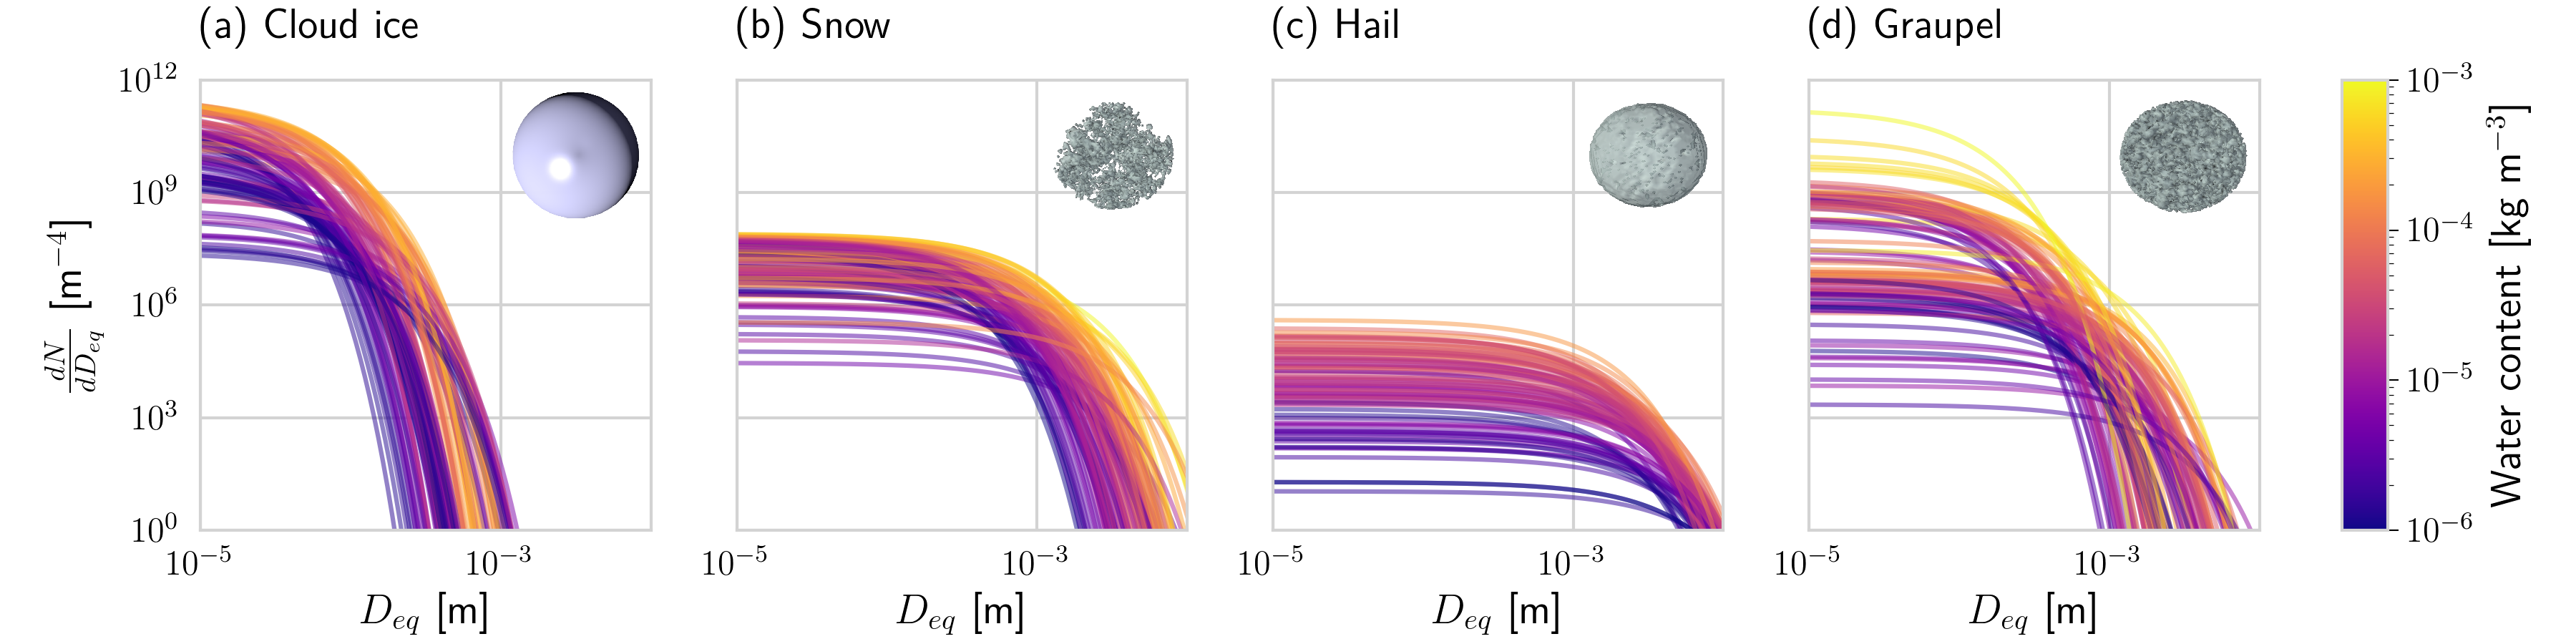
\includegraphics[width = \textwidth]{../plots/gem_psds.png}
\caption{Realizations of particle size distributions from the test scenes used
  in this study. The particle number concentration is plotted with respect to
  the volume-equivalent diameter $D_\text{eq}$. Shown are the PSDs corresponding
  to 100 randomly chosen grid points with a water content higher than
  $10^{-6}\ \unit{kg\ m^{-3}}$. Line color encodes the corresponding water
  content. Inlets display visualizations of the particle shape assumed for each
  hydrometeor species.}
\label{fig:gem_psds}
\end{figure}

\subsection*{Reviewer comment 8}

4) Units of standard deviation of Z. The authors are reiterating common mistakes/typos present in literature,
even when errors are highlighted. dBZ-dBZ is dB, that's the nature of logarithmic units! 

\subsubsection*{Author response}

We would like to thank the reviewer for pointing and will correct this in the
revised manuscript.

\subsubsection*{Changes in manuscript}
\begin{change}[138]
 The minimum sensitivity is set to be $-30\ \unit{dBZ}$ and the noise at each
 range gate is modeled to be independent with standard deviation \DIFdelbegin
 \DIFdel{$0.5\ \unit{dBZ}$}\DIFdelend \DIFaddbegin
 \DIFadd{$0.5\ \unit{dB}$}\DIFaddend .
\end{change}

\subsection*{Reviewer comment 9}
5) Eq.3 : another wrong equation. Not sure what the authors are doing here but
it is simple algebra, the equation is clarly wrong because there is no factor pi
involved (see
https://agupubs.onlinelibrary.wiley.com/doi/epdf/10.1029/2018JD028603).

\subsubsection*{Author response}

The work referenced by the referee does in fact employ a similar transform. The
transform in the referenced study however employs the inverse tangens, while we
employ the inverse \textit{hyperbolic} tangens. Using \textit{simple algebra} it
can be easily seen that a factor of $\pi$ is not required in this case.

The plot given below shows the relation between the quantities $x$ and $RH$ in
the equation and it illustrates that the transformation does what it is expected
to do: Map arbitrary values of $x$ to the range $[0.0, 1.2]$. We therefore do
not see what the referee expects us to correct here.

\begin{figure}
 \includegraphics[width=0.5\textwidth]{../plots/atanh}
 \caption{Plot of the relation between relative humidity values and the
   transformed quantity $x$.}
 \label{fig:atanh}
\end{figure}

\subsection*{Reviewer comment 10}


6) Eq.6 is another example of very confused terminology (the numerator is not a
cross section!! efficiency is usually used for other scattering quantities)

\subsubsection*{Author response}

I don't really have an idea what he means there. I do think what I wrote
is right, but I may be missing something.


\subsection*{Reviewer comment 11}

7) Fig.4 also does not make much sense to me (if you are normalising by IWC you
should not plot it in the x-axis).

\subsubsection{Author response}

This is a false statement. As the plots show, there is a non-linear dependency
between water content and scattering properties and normalization therefore does
not cancel the dependency of the mass backscattering coefficient on the water
content. Moreover, normalization is required to make the differences between
different particles discernable in the plot, which would otherwise be dominated
by the strong increase of the backscattering coefficient with bulk mass.

\subsection*{Reviewer comment 11}

8) Fig.7 y-label panel b) That is not IWP but a ratio of IWP_ret/IWP/true. Re-label.

\subsubsection{Author response}

We will relabel the figure according to the referees suggestions.


\subsection*{Reviewer comment 12}

9) Units of IWC in Fig.14 are wrong.

\subsubsection{Author response}

We thank the referee for pointing out this inconsistency and will correct it in the
revised manuscript.

\subsection*{Reviewer comment 13}

Proper scrutiny must be paid by the authors in the third round (and I would
specifically urge the more expert co-authors for providing such scrutiny that
was clearly missing in the previous two rounds! ). This means not simply
addressing the issues mentioned above but properly perusing thoroughly the whole
paper! Please avoid generic sentences.

\subsubsection{Author response}

We thank the referee for this valuable comment and look forward to a more expert
referee in the next round.

\subsection*{Reviewer comment 13}

1) I am still convinced about some major issues related to the selection of the
scene. The key strength of the combination should be in ice clouds and
mixed-phase but no clear message are coming out of this study on this (i.e. what
king of cloud-LWP can we retrieve with confidence? how important is to know the
location of the SLWC layer?). Profiles with high density ice and rain underneath
are much more complicated and certainly should not be the target of such a suite
of instruments (but they occupy a large fraction of your scene). The only
semi-quantitative statements is indeed present in the conclusions ``While
observations at currently available microwave frequencies provide information
complementary to that from a radar only for thick clouds with very large
particles ...'' and is actually based on your Fig.5 (no retrieval involved).

\subsection*{Author response}

As pointed out above, we have justified the selection of the test scenes in our
previous response. The presented scenes contain a wide range of different cloud
formations, which we chose over cherry picking specific scenes where the
combined retrieval works well. We did this in order to provide a more balanced
view over the potential and limitations of the combined retrieval.

The referee goes on to request a more accurate assessment of the performance
of the LWC retrieval, although we mention clearly that the main focus of our
article is the retrieval of ice hydrometeors. The assessment of these specific
cases is therefore out the scope of this article. We would also like to contrast
that with the referees comments made in the first article that complained about
the length of the manuscript.

It is true that we refrain from making absolute statements on the performance of
the combined retrieval. This is because our intention was never to develop a
production-ready implementation and give accurate performance estimates of such
a retrieval, which we clearly state in the section on the limitations of the
study. Since this is study is based purely on simulations the reliability of
such an analysis would anyways be questionable.

The main points of this comment have not been raised in the referee's first review
and were therefore impossible for us to address. Moreover, the out-of-scope nature of the
request gives the impression that the referees is not interested in actually improving
the study but instead simply wants to delay or hinder its publication.


\subsection*{Reviewer comment 14}

2) Fig.3 and retrieval grid: the definition of the retrieval grid must be
different if you consider a radiometer only or a retrieval including the radar.
The advantage of a radar is indeed to produce a cloud mask first (actually with
the sensitivity you have used all clouds are practically detected by the radar).
So I really do not understand how it is possible to see IWC in Fig,.7 panel e)
and f) where there are no clouds (this magically disappear in Fig.10???). On the
other hand I am also curious to know how with a radiometer-only retrieval you
can constrain the cloud top like you are doing.

\subsection*{Author response}

As it is explained in the manuscript, the retrieval grids for radar and radiometer retrievals
are the same but to regularize the radiometer retrieval the passive-only retrieval
uses a higher correlation length in the a priori covariance matrix. The referee is
invited to validate our claims by running the retrieval himself the code of which
is publicly accessible.

The contradicting data that the reviewer points out in  Fig. 10, is due to an error in the
masking threshold applied, which was chosen at $5\cdot 10^{-6}\unit{kg \ m^{-3}}$ and not
$1\cdot 10^{-6}\unit{kg \ m^{-3}}$. However, the reviewer is in incorrect in his assumption
that we use the radar signal to apply a cloud mask, which we have not pursued here.

\chapter{Marked-up differences}

\bibliographystyle{copernicus}
\bibliography{references}

\end{document}
